\subsection{Фазы планет и спутников}

\term{Фаза} планеты (спутника)~--- отношение площади освещённой  части видимого диска ко всей его площади.
Фаза рассчитается по следующей формуле:\begin{equation}
\Phi = \frac{1 + \cos \phi}{2} = \cos^2 \frac{\phi}{2},
\end{equation}
где $\varphi$~--- \term{фазовый угол} --- угол между лучом света, падающим от Солнца на планету, и лучом, отразившимся от неё в сторону наблюдателя (Рис.~\ref{fig:phase-angel-scheme}). Фаза объекта может принимать значения от 0 до 1.
\begin{figure}[h!]
\centering
\includegraphics[width = .49\tw]{phase-angle}
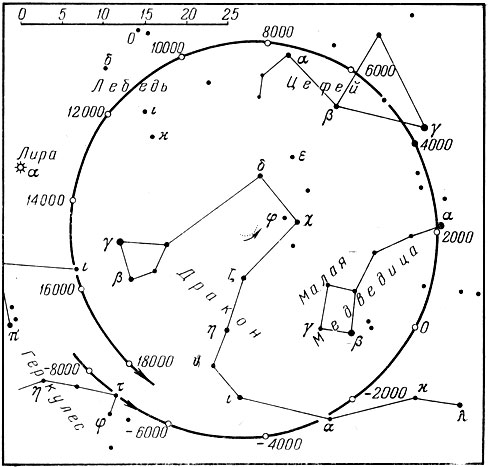
\includegraphics[width = .49\tw]{Precess}
\caption{Фазовый угол}
\label{fig:phase-angel-scheme}
\end{figure}